\usetikzlibrary{shapes.geometric, arrows.meta, positioning, calc, shadows}
\tikzset{
  base/.style = {
    draw, thick, minimum height=1.2cm, minimum width=3.6cm,
    font=\sffamily, text centered, rounded corners=4pt, drop shadow
  },
  input/.style = {
    base, fill=blue!10, draw=blue!60
  },
  process/.style = {
    base, fill=green!10, draw=green!50!black
  },
  output/.style = {
    base, fill=red!10, draw=red!60
  },
  arrow/.style = {
    thick, -{Latex[length=3mm]}, line cap=round,
    shorten >=2pt
  }
}

\centering
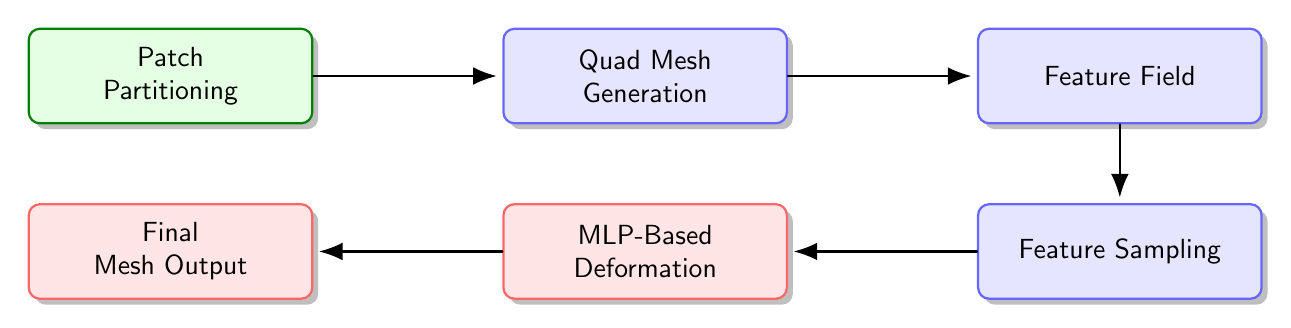
\begin{tikzpicture}[
  node distance = 1cm and 2.4cm,
  every node/.style = {align=center}
  ]

  % Top row (left to right)
  \node[process] (partition) {Patch\\Partitioning};
  \node[input, right=of partition] (quadmesh) {Quad Mesh\\Generation};
  \node[input, right=of quadmesh] (featurefield) {Feature Field};

  % Bottom row (right to left)
  \node[input, below=of featurefield] (sampling) {Feature Sampling};
  \node[output, left=of sampling] (mlp) {MLP-Based\\Deformation};
  \node[output, left=of mlp] (render) {Final\\Mesh Output};

  % Arrows (top row)
  \draw[arrow] (partition) -- (quadmesh);
  \draw[arrow] (quadmesh) -- (featurefield);

  % Arrows (down and bottom row leftward)
  \draw[arrow] (featurefield) -- (sampling);
  \draw[arrow] (sampling) -- (mlp);
  \draw[arrow] (mlp) -- (render);

\end{tikzpicture}

\captionof{figure}{Schematic of the processing pipeline. Patch partitioning and quad mesh generation lead to a feature field construction. The field is sampled, deformed using a Multi-Layer Perceptron (MLP) and converted into the final mesh output.}
\label{fig:teaser}
  